\FloatBarrier  % Beendet das Wrapping vor der nächsten Section
\section{Erste Sequenz}
 %works? keep whitespace
\begin{wrapfigure}{R}{0.5\textwidth}
	\centering
	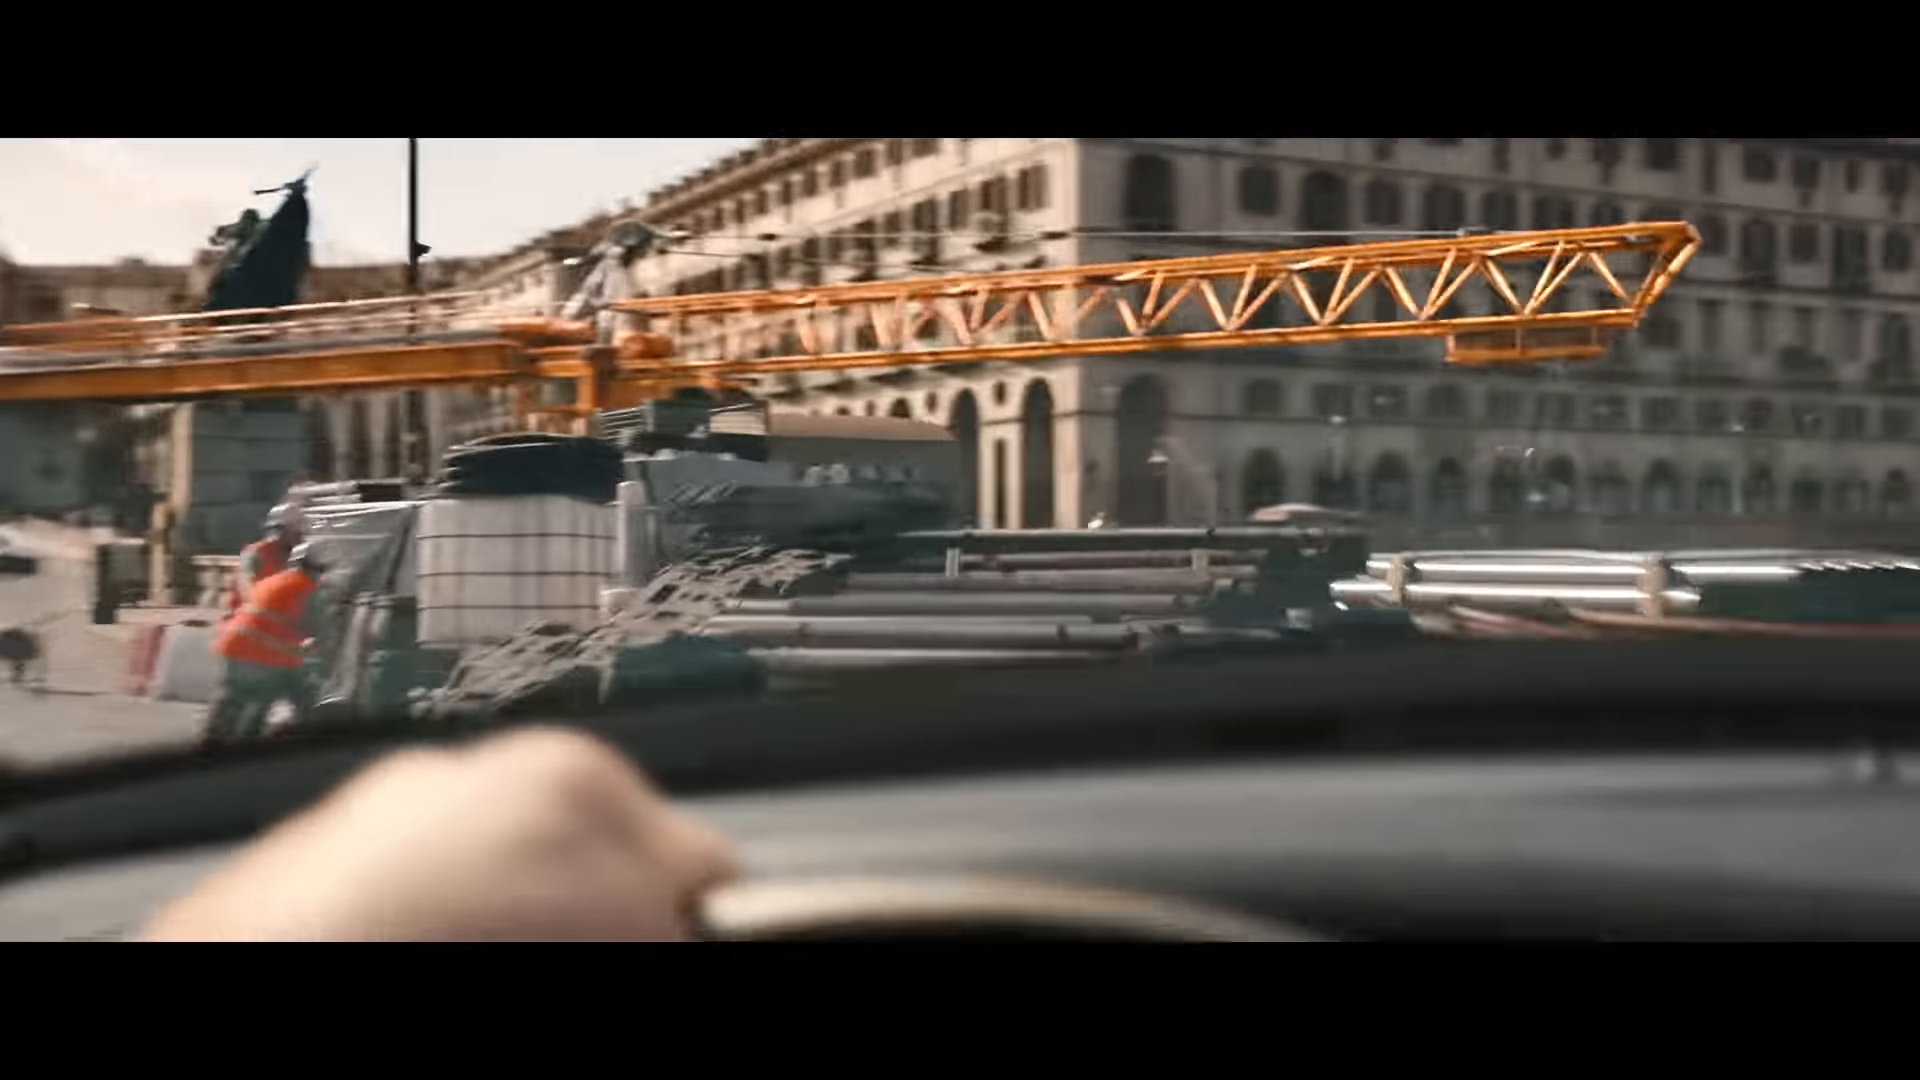
\includegraphics[width=0.48\textwidth]{resources/seq2/00_xy-angle_dom-pov.png}
	\vspace*{-5mm}
	\begin{flushright}
		{\scriptsize\textcopyright\ 2023 Universal Pictures}
	\end{flushright}
	
	\captionsetup{
		labelfont=bf,
		textfont=footnotesize,
		skip=0pt
	}
	\caption{Screenshot Fast X: Dom fährt auf Rampe zu}
	\label{fig:00_xy-angle_dom-pov}
	%\vspace{-10pt}
\end{wrapfigure}
Doms Sprung von der provisorischen Stangenrampe markiert den Anfang der Berechnungen. \hyperref[fig:00_xy-angle_dom-pov]{Abbildung~\ref*{fig:00_xy-angle_dom-pov}} zeigt den Blickpunkt Doms beim Zusteuern auf die Rampe. Aufgrund der Länge der Stangen hat er freie Wahl über den horizontalen Winkel, mit dem er auf diese Auffahrt trifft.
\\
Der Abschusswinkel des Autos bestimmt jedoch maßgeblich wo, und ob Dom überhaupt mit dem Ausleger kollidiert.
\\
Da auf das Auto senkrecht zur Flugrichtung keinerlei Kräfte wirken, und sich das Geschoss somit aus der Draufsicht annähernd geradlinig bewegt, lässt sich diese eigentlich 3-dimensionale Trajektorie einfach über eine 2-dimensionale Parabel eines schrägen Wurfs beschreiben.

\subsection{Rampenwinkel} %im kontext
\begin{wrapfigure}{l}{0.4\textwidth}
	\centering
	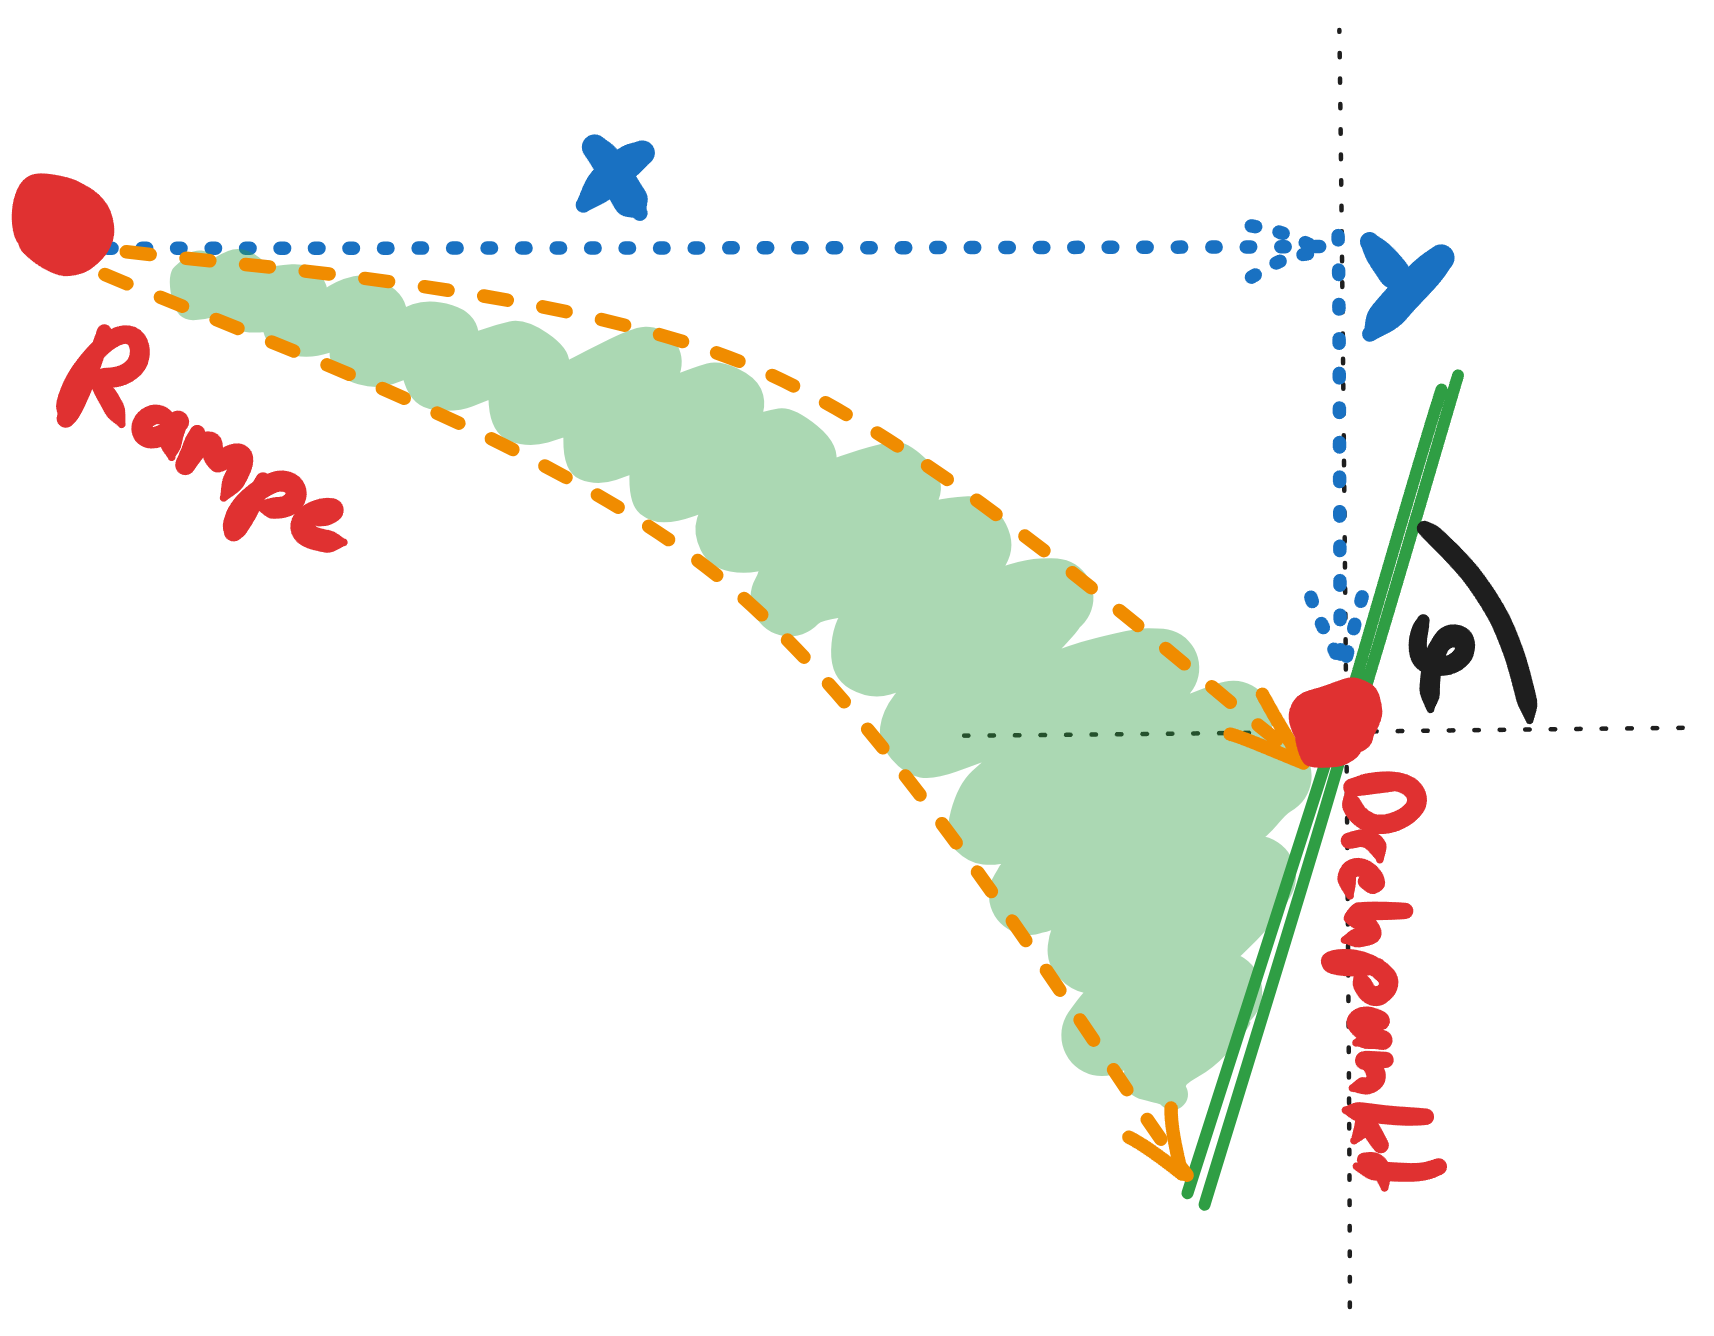
\includegraphics[width=0.38\textwidth]{resources/seq2/sketch-simple.png}
	\vspace*{-5mm}
	\begin{flushright}
		{\scriptsize Eigenkreation; Gezeichnet in Excalidraw}
	\end{flushright}
	
	\captionsetup{
		labelfont=bf,
		textfont=footnotesize,
		skip=0pt
	}
	\caption{Einfache Skizze der Sequenz in Obersicht}
	\label{fig:01_xy-angle_sketch-simple}
	%\vspace{-10pt}
\end{wrapfigure}
Der Geometrie des Sprungs ist in \hyperref[fig:01_xy-angle_sketch-simple]{Abbildung~\ref*{fig:01_xy-angle_sketch-simple}} simpel skizziert worden. Der rote Punkt im linken oberen Eck steht für den Absprung des Autos, den Punkt ab dem die Reifen den Boden verlassen und die Flugbahn beginnt.
Die Zeichnung stellt den Sachverhalt aus der Obersicht dar. Die Flugbahn wird daher nicht nur aus der zur Erdoberfläche parallelen XY-Ebene, sondern zu einem Teil auch aus der %für die Höhe zuständige
XZ-Ebene betrachtet. 
Dadurch ergibt sich die leichte Krümmung der orange gestrichelten Flugbahn des Autos.\\
Der zweite rote Punkt steht für den Drehpunkt des Turmkrans und ist im Echtwelt-Äquivalent mit dem Drehkranz auf dem Gittermastturm gleichzusetzen. 
Über den Betrag der Differenz der jeweiligen X und Y Komponente der Koordinaten, werden die Punkte in Relation gesetzt. Da die beiden Punkte nur über ihre relativen Abstände definiert sind, wäre es hier falsch von einem Koordinatensystem zu sprechen, viel eher befinden wir uns in einem metrischen Raum \parencite{MetrischerRaumWiki}. %todo 
\\
Der grüne Balken der durch besagten Punkt verläuft ist dementsprechend das Oberschwenkwerk. Der hintere Teil der Linie, der mit der X-Achse den Drehwinkel $\varphi$ einschließt, trägt im Film das Gegengewicht.
Dom muss mit dem vorderen Teil, dem Ausleger, kollidieren um den Kran in die richtige Drehbewegung zu versetzen.
\\
Der grün-markierte Bereich zwischen den beiden Pfeilen kennzeichnet alle für einen erfolgreichen Stoß gültigen Winkel




\subsection{Berechnung}

\begin{wrapfigure}{R}{0.5\textwidth}
	\centering
	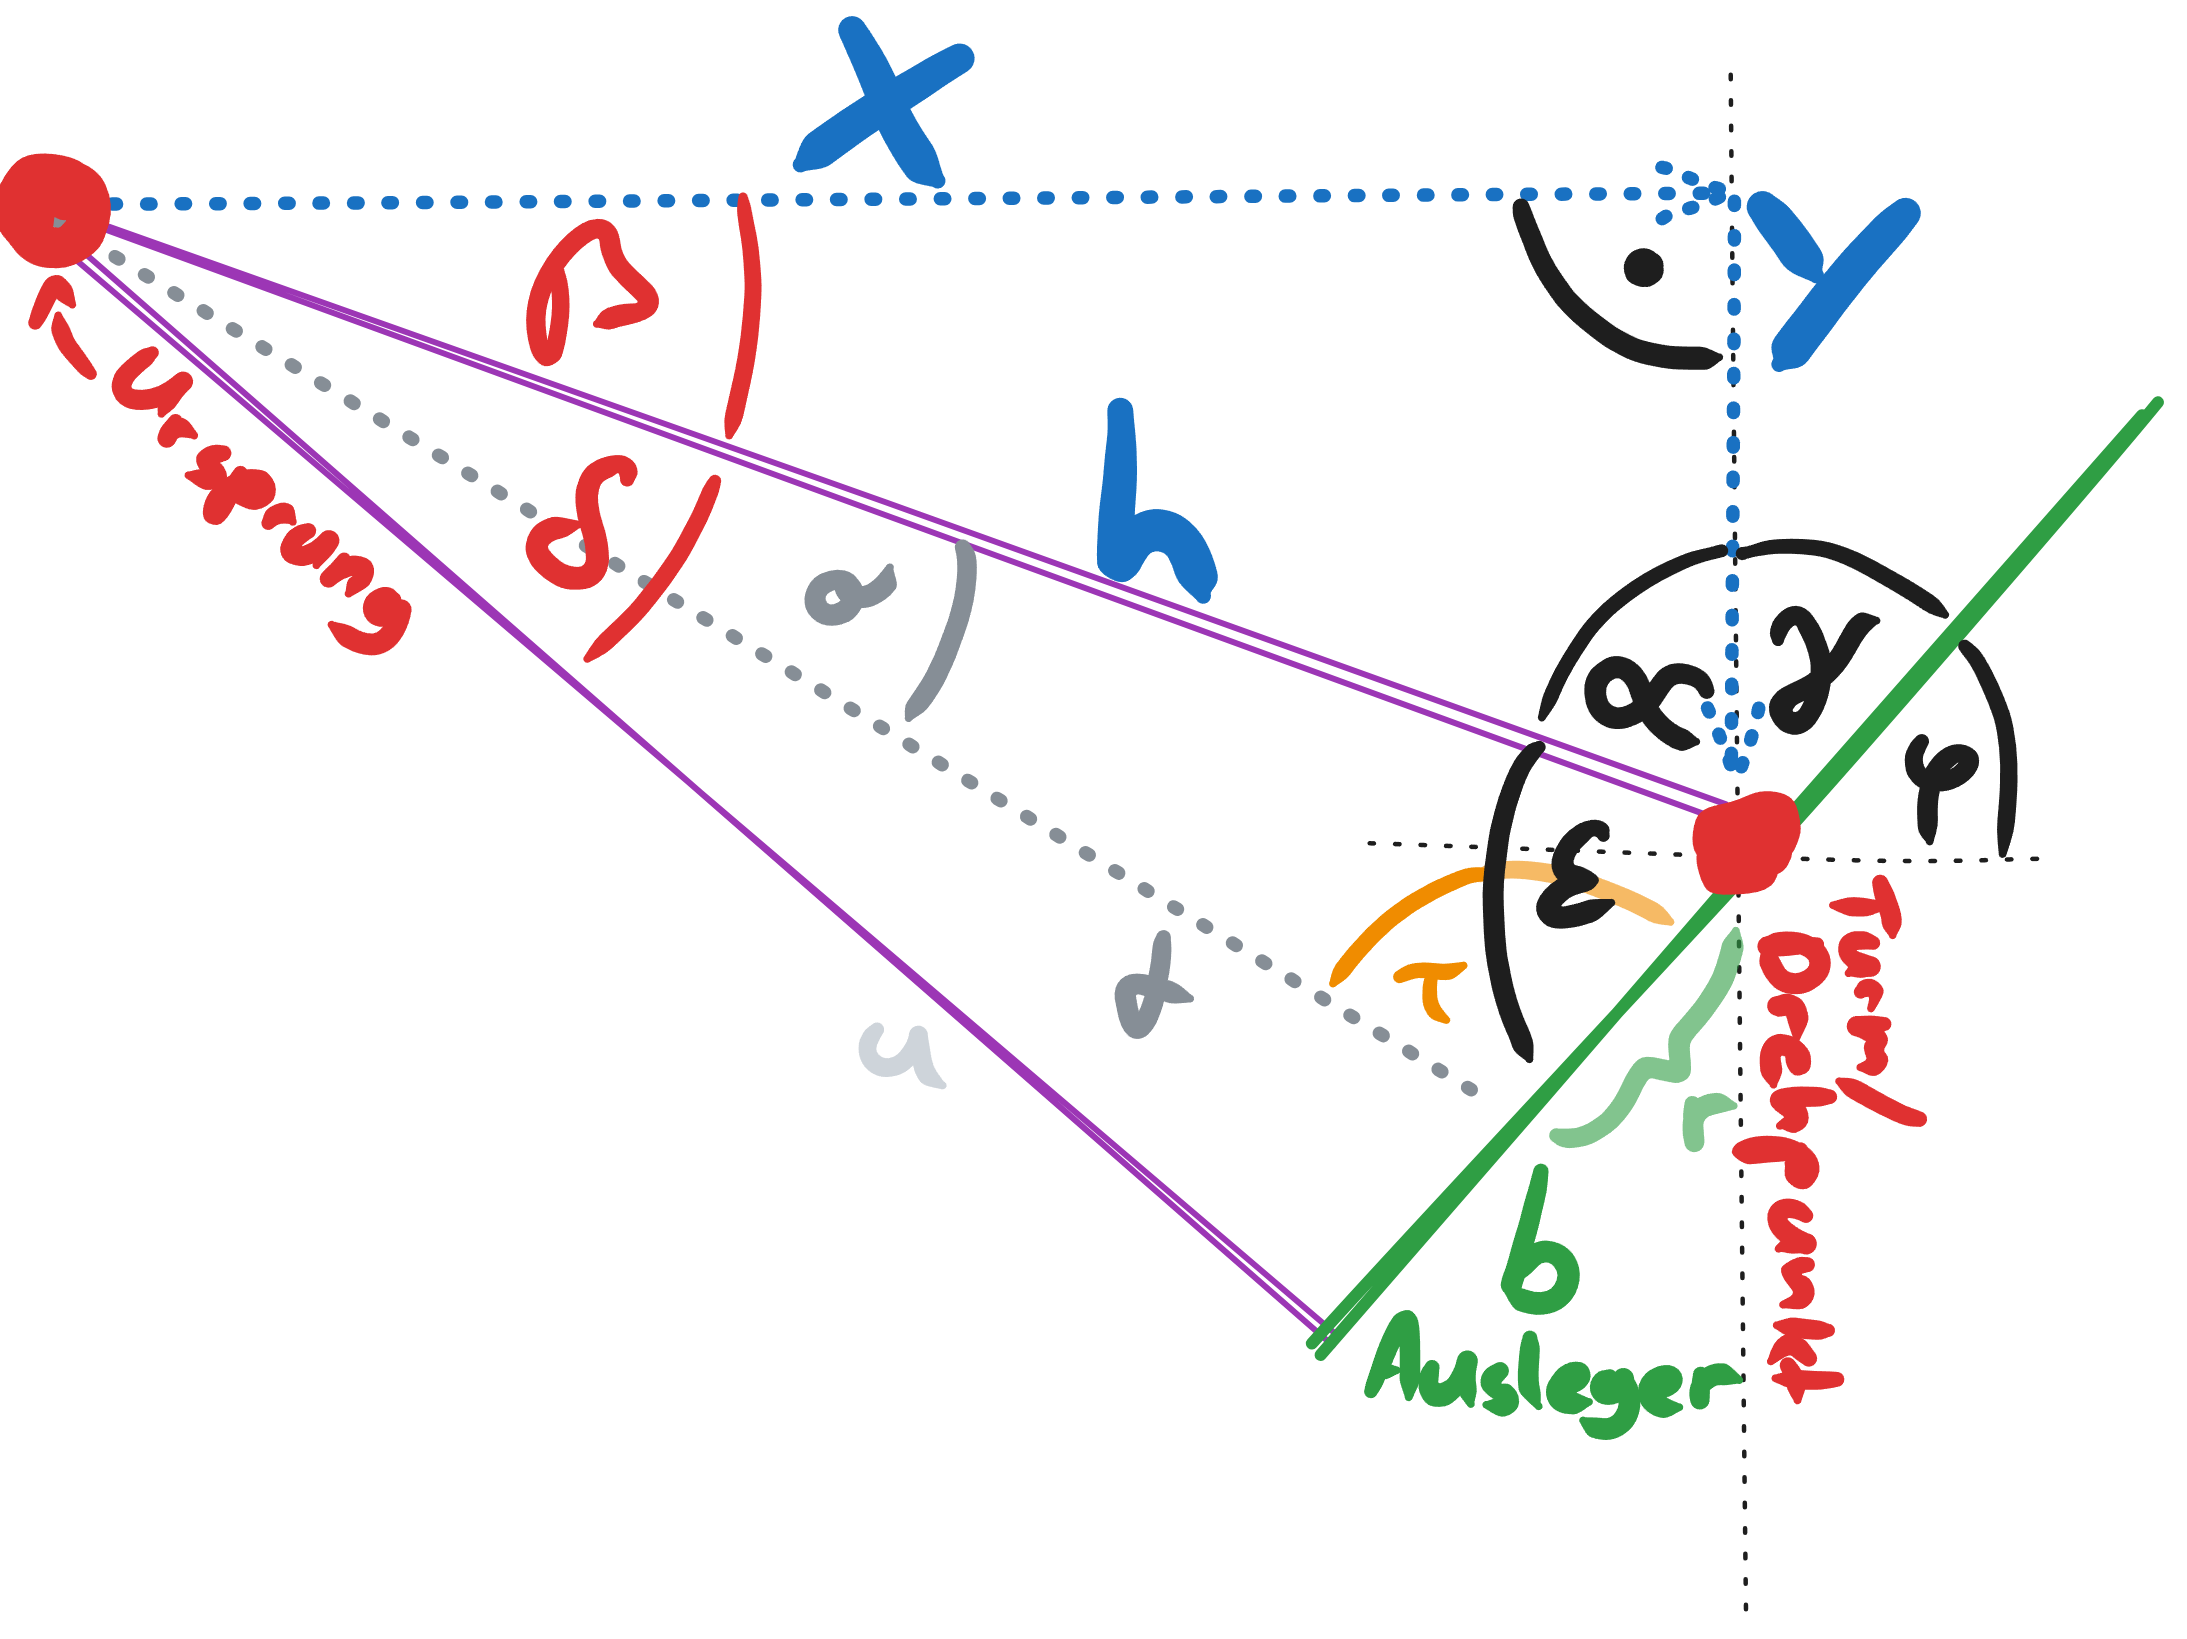
\includegraphics[width=0.48\textwidth]{resources/seq2/sketch-detailed.png}
	\vspace*{-10mm}
	\begin{flushright}
		{\scriptsize Eigenkreation; Gezeichnet in Excalidraw}
	\end{flushright}
	
	\captionsetup{
		labelfont=bf,
		textfont=footnotesize,
		skip=0pt
	}
	\caption{Detaillierte Skizze der Sequenz in Draufsicht}
	\label{fig:02_xy-angle_sketch-detailed}
	%\vspace{-10pt}
\end{wrapfigure}
Um nun das gesamte System vollständig zu beschreiben und Unbestimmten zu eliminieren, muss man sich der grundlegenden Gesetze der Trigonometrie bedienen. Man kann schritt f